\chapter{Desarrollo de pruebas y análisis de resultados.}
\section{Entorno de pruebas.}
Para el desarrollo de las pruebas, mi ordenador personal ha sido utilizado. Las especificaciones ténicas relevantes del mismo son:

\begin{itemize}
\item \textbf{Placa Base:} MSI B450M Bazooka
\item \textbf{Sistema Operativo:} Windows 10 64 bits
\item \textbf{CPU:} AMD Ryzen 5 2600X
\item \textbf{RAM:} Kingston HyperX Fury Black DDR4 2400 MHz PC4-19200 8GB CL15
\item \textbf{GPU}: \underline{Zotac GeForce GTX 1060 AMP! Edition}
\subitem \textbf{Núcleos CUDA}: 1280
\subitem \textbf{Frecuencia del procesador:} 1556 MHz (1771 MHz Boost)
\subitem \textbf{Frecuencia de la memoria:} 8 GHz
\subitem \textbf{Memoria}: 6 GB DDR5
\subitem \textbf{Bus de memoria:} 192-bit
\subitem \textbf{Compute Capability:} 6.1

\end{itemize}

\newpage

\section{Conjuntos de datos utilizados.}

Durante la fase de desarrollo del mapa autoorganizado hemos utilizado el conjunto de datos de las \textbf{caras de Olivetti}, creado por \textit{AT\&T Laboratories Cambridge} y descargada a través del paquete de Python \textit{scikit-learn} \cite{olivetti}. Dicho conjunto de imágenes consiste en 400 imágenes de 40 sujetos en escala de grises. Cada muestra son los valores de intensidad de cada píxel con un valor normalizado entre 0 y 1. Además, se proporciona una etiqueta que indica a qué sujeto pertenece cada imagen pero para los propósitos de nuestro modelo de aprendizaje no supervisado la misma no será utilizada. Las imágenes están en una versión cuadrada de 64x64 píxeles dándonos un total de 4096 valores de intensidad por muestra. \\

Durante la fase de desarrollo del árbol de decisión hemos utilizado dos conjuntos de datos de problemas de clasificación binaria: \textbf{Spambase} y \textbf{MAGIC Gamma Telescope}.\\

\textbf{Spambase} \cite{spambase} es un conjunto de 4601 muestras con 57 atributos. El objetivo en este conjunto de muestras es diferenciar correos no deseados (\textit{spam}) de correos deseados en función de los 56 atributos numéricos basados en el contenido del correo electrónico asociado a la muestra.\\

\textbf{Magic Gamma Telescope} \cite{magic04} es un conjunto de 19020 muestras con 11 atributos. Los datos de este conjunto fueron obtenidos en un experimento con un telescopio especial para observar rayos gamma de alta energía. El objetivo es diferenciar imágnes tomadas por el telescopio y preprocesadas de estas muestras generadas por rayos gamma (\textit{signal}) de las de rayos cósmicos en la capa superior de la atmósfera (\textit{background}). Los datos de este conjunto fueron generados a partir de simulaciones de Monte Carlo.\\

Para evaluar el rendimiento de ambos modelos para conjuntos de \textit{Big Data} hemos utilizado \textbf{SUSY} \cite{susy}. Este conjunto de datos contiene 5 millones de muestras con 18 atributos, que se generó a partir de un experimento de física en el que también se intenta diferencia un proceso que genera partículas supersimétricas (\textit{signal}) de otro proceso que no las genera (\textit{background}). En el caso del mapa autoorganizado la clase de salida es ignorada. De manera similar al anterior, los datos del conjunto fueron generadors a partir de simulaciones de Monte Carlo.


\section{Experimentos para evaluar el mapa autoorganizado.}
En el caso del mapa autoorganizado tanto la versión como para CPU como para GPU ejecutan el mismo algoritmo por lo que la métrica de interés durante las ejecuciones realizadas es el tiempo de ejecución. En primer lugar, durante la fase de desarrollo usamos el conjunto de las caras de \textit{Olivetti}, que nos permitió comprobar de manera empírica y gráfica que los resultados son correctos. En caso de funcionar, correctamente generamos un conjunto de imagenes con la misma dimensión del mapa que son o se parecen a algunas de las caras de los sujetos y donde las imágenes más parecidas se encuentran próximas las unas con las otras. \\

\textit{NOTA: Pendiente de ejecutar un ejemplo representantivo para un mapa de neuronas apropiado para un papel A4.}

Posteriormente, para evaluar la capacidad del algoritmo ante un conjunto de mayores dimensiones utilizamos SUSY. Para este experimento ignoramos las etiquetas de salida y utilizamos para un mapa de neuronas de 8 filas y 7 columnas con los parámetros de control $\tau$ a 10 y $\sigma_0$ a 4. El algoritmo lo ejecutamos durante 10 iteraciones y realizamos 5 repeticiones de cada experimento para tomar una medida de tiempo promedio más fiable. En este experimento no nos limitamos sólo a evaluar con el conjunto de muestras al completo (5 millones de muestras) sino que probamos desde medio millón de muestras hasta el conjunto completo aumentando en cada paso medio millón de muestras. Los resultados de este experimentos los podemos observar en las siguientes figuras.\\

\begin{figure}[ht]
\centering
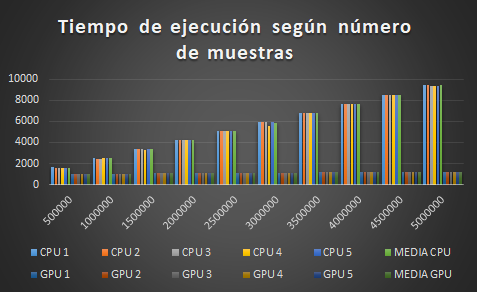
\includegraphics[scale=0.8]{imagenes/tiempossusysom.png}
\caption{Tiempos de ejecución del mapaautoorganizado para SUSY.}
\label{img:somsusy}
\end{figure}

\begin{figure}[ht]
\centering
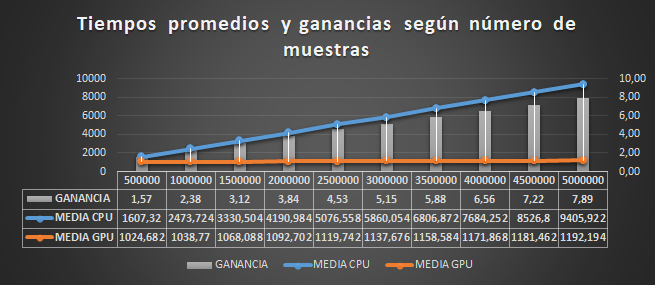
\includegraphics[scale=0.8]{imagenes/gananciassom.png}
\caption{Ganancias del mapaautoorganizado para SUSY.}
\label{img:gananciassomsusy}
\end{figure}

En este experimento podemos ver cómo evoluciona la ganancia de nuestra implementación que combina \textit{CUDA} y \textit{Spark} para evaluar un número de muestras elevado. En primer lugar, hemos de tener en cuenta que, al leer el archivo CSV, \textit{Spark} generó un \textit{RDD} con 72 particiones, es decir, 6 particiones para cada uno de los 12 núcleos (6 físicos y 6 lógicos) de nuestro AMD Ryzen 5 2600X. A la hora de evaluar con la GPU hemos mantenido el mismo número de particiones, por lo que en al evaluar 500000 en realidad estamos realizando 72 ejecuciones independientes del algoritmo y combinando todos los resultados obtenidos. Mientras que la generación de múltiples particiones facilita que los conflictos que se puedan generar para realizar las operaciones atómicas sean menores, resulta claro que conforme aumentamos el tamaño de la muestra obtenemos ganancias considerablemente mayores, como podemos observar en la figura \ref{img:gananciassomsusy}. Es por ello, que, a la hora de utilizar este algoritmo en la práctica hemos de concluir que hemos de exprimir al máximo las capacidades de la memoria del dispositivo CUDA para obtener las mejores ganancias. En nuestro caso, en el ejemplo más complejo que hemos evaluado obtenemos un tiempo de ejecución casi 8 veces más rápido en nuestra GTX 1060 que en los 12 cores de nuestro Ryzen.

\newpage
\section{Experimentos para evaluar el árbol de decisión.}
Para los experimentos relaciones con estos problemas de clasificación tenemos en cuenta dos métricas: el tiempo de ejecución y la precisión (porcentaje de predicciones correctas).\\

En primer lugar, durante el proceso de desarrollo, se empezó a evaluar la creación de un único árbol con profundidad limitada entre la implementación desarrollada y la implementación de Spark. Hemos de destacar, antes de comentar los resultados obtenidos, que, a diferencia del modelo anterior, el algoritmo utilizado para el cálculo en la CPU y el creado en CUDA no hacen lo mismo (el nuestro esta basado en una búsqueda exhaustiva de puntos de corte y el de Spark en una discretización por cuantiles y el uso de histogramas) aunque ambos generen un árbol de decisión. Los resultados obtenidos fueron generados mediante un proceso de validación cruzada \textit{leave-one out} con 10 particiones, es decir se generaron 10 particiones aleatorias de los datos y, en cada iteración, una es seleccionada para comprobar la precisión del modelo obtenido y el resto para entrenarlo, de tal manera que todas las particiones son utilizada para comprobar la calidad del modelo generado por el resto de ellas. Los resultados obtenidos de la validación cruzada son el promedio de estas iteraciones.
\newpage
\subsection{Tablas de resultados para la generación de un único árbol.}
\begin{table}[ht]
\begin{tabular}{@{}r|c|c|c|c|@{}}
\cmidrule(l){2-5}
\multicolumn{1}{c|}{\textbf{}}                      & \multicolumn{4}{c|}{\textit{\textbf{SPAMBASE (4601 muestras, 57 atributos)}}}                                                                                                                                         \\ \cmidrule(l){2-5} 
\multicolumn{1}{l|}{}                               & \multicolumn{2}{c|}{\textit{\textbf{CUDA}}}                                                               & \multicolumn{2}{c|}{\textit{\textbf{SPARK}}}                                                              \\ \midrule
\multicolumn{1}{|l|}{\textit{\textbf{Profundidad}}} & \textit{\textbf{\begin{tabular}[c]{@{}c@{}}Tiempo \\ (s)\end{tabular}}} & \textit{\textbf{\begin{tabular}[c]{@{}c@{}}Precisión \\ (\%)\end{tabular}}} & \textit{\textbf{\begin{tabular}[c]{@{}c@{}}Tiempo \\ (s)\end{tabular}}} & \textit{\textbf{\begin{tabular}[c]{@{}c@{}}Precisión \\ (\%)\end{tabular}}} \\ \midrule
\multicolumn{1}{|r|}{\textit{\textbf{4}}}           & \textbf{2,58}                                     & 88,13                                                 & 6,47                                              & \textbf{88,64}                                        \\ \midrule
\multicolumn{1}{|r|}{\textit{\textbf{5}}}           & \textbf{2,92}                                     & 85,7                                                  & 6,48                                              & \textbf{90,77}                                        \\ \midrule
\multicolumn{1}{|r|}{\textit{\textbf{6}}}           & \textbf{4,44}                                     & 86,2                                                  & 6,6                                               & \textbf{91,14}                                        \\ \midrule
\multicolumn{1}{|r|}{\textit{\textbf{7}}}           & \textbf{7,32}                                     & 89,72                                                 & 6,75                                              & \textbf{91,9}                                         \\ \midrule
\multicolumn{1}{|r|}{\textit{\textbf{8}}}           & 10,81                                             & 90,15                                                 & \textbf{6,84}                                     & \textbf{91,95}                                        \\ \midrule
\multicolumn{1}{|r|}{\textit{\textbf{9}}}           & 12,15                                             & 85,8                                                  & \textbf{6,9}                                      & \textbf{92,29}                                        \\ \bottomrule
\end{tabular}
\caption{Validación cruzada para árbol de decisión en spambase.}
\label{tab:spamtree}
\end{table}

\begin{table}[ht]
\begin{tabular}{@{}r|c|c|c|c|@{}}
\cmidrule(l){2-5}
\multicolumn{1}{c|}{\textbf{}}                      & \multicolumn{4}{c|}{\textit{\textbf{MAGIC (19020 muestras, 11 atributos)}}}                                                                                                                                                                                                                                   \\ \cmidrule(l){2-5} 
\multicolumn{1}{l|}{}                               & \multicolumn{2}{c|}{\textit{\textbf{CUDA}}}                                                                                                           & \multicolumn{2}{c|}{\textit{\textbf{SPARK}}}                                                                                                          \\ \midrule
\multicolumn{1}{|l|}{\textit{\textbf{Profundidad}}} & \textit{\textbf{\begin{tabular}[c]{@{}c@{}}Tiempo \\ (s)\end{tabular}}} & \textit{\textbf{\begin{tabular}[c]{@{}c@{}}Precisión \\ (\%)\end{tabular}}} & \textit{\textbf{\begin{tabular}[c]{@{}c@{}}Tiempo \\ (s)\end{tabular}}} & \textit{\textbf{\begin{tabular}[c]{@{}c@{}}Precisión \\ (\%)\end{tabular}}} \\ \midrule
\multicolumn{1}{|r|}{\textit{\textbf{4}}}           & \textbf{0,36}                                                           & 79,37                                                                       & 6,42                                                                    & \textbf{81,41}                                                              \\ \midrule
\multicolumn{1}{|r|}{\textit{\textbf{5}}}           & \textbf{0,65}                                                           & 80,99                                                                       & 6,48                                                                    & \textbf{81,71}                                                              \\ \midrule
\multicolumn{1}{|r|}{\textit{\textbf{6}}}           & \textbf{1,17}                                                           & 81,77                                                                       & 6,58                                                                    & \textbf{83,59}                                                              \\ \midrule
\multicolumn{1}{|r|}{\textit{\textbf{7}}}           & \textbf{2,09}                                                           & 83,87                                                                       & 6,71                                                                    & \textbf{84,23}                                                              \\ \midrule
\multicolumn{1}{|r|}{\textit{\textbf{8}}}           & \textbf{3,52}                                                           & 84,1                                                                        & 6,81                                                                    & \textbf{84,55}                                                              \\ \midrule
\multicolumn{1}{|r|}{\textit{\textbf{9}}}           & \textbf{5,77}                                                           & 84,2                                                                        & 7,05                                                                    & \textbf{84,73}                                                              \\ \bottomrule
\end{tabular}
\caption{Validación cruzada para árbol de decisión en MAGIC.}
\label{tab:magictree}
\end{table}
\newpage

\subsection{Análisis de los resultados para la generación de un único árbol.}
\begin{figure}[ht]
\centering
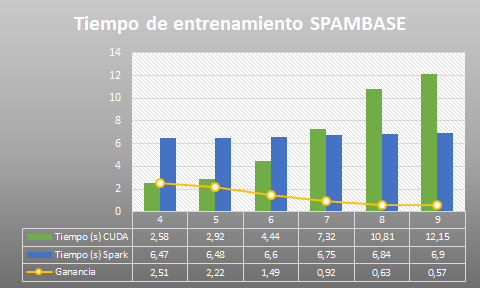
\includegraphics[scale=1.0]{imagenes/spambase_times.png}
\caption{Tiempo de entrenamiento y ganacia según profundidad en Spambase.}
\label{img:spambasetimes}
\end{figure}
En la figura \ref{img:spambasetimes} podemos observar cómo evolucionan los tiempos de ejecución del modelo para CPU (en azul) y CUDA (en verde) según vamos aumentando la profundidad de los árboles generados empezando en cuarto nivel de profundidad y terminando en el noveno. Podemos concluir con facilidad que el rendimiento de la implementación en CUDA empeora considerablemente conforme aumentamos los niveles de profundidad, incluso llegando a ser más lento que la versión en CPU de \textit{Spark}, factor que resulta razonable pues, conforme vamos aumentando dicho nivel más kernels han de ser lanzados y el número de muestras en cada uno va a ser inferior pudiendo llegar a ser incapaz de aprovechar la capacidad de procesamiento que tienen los núcleos de CUDA por ejemplo sin el nodo no hay suficientes elementos para utilizar todas las hebras de un bloque o siquiera las de un \textit{warp}, así como la reorganización de los datos en la memoria que sigue siendo una operación bastante costosa, aunque no haga falta aplicar de nuevo un algoritmo de ordenación, que ocurre en cada nivel. \\

La generación de un árbol de decisión para Spambase expone los dos problemas principales cuando utilizamos este algoritmo: tener un número de muestras relativamente reducido y una gran cantidad de listas de atributos. Si tenemos un número de muestras más o menos reducido, en este caso tenemos 4600 muestras, el nivel de profundidad én el que la utilización de la GPU de manera efectiva decae considerablemente se alcanza antes. Por otro lado, el elevado número de atributos (56 más la etiqueta de salida) implica la generación de 56 listas de atributos que generan tanto un \textit{overhead} en la complejidad espacial del modelo en la GPU como en la cantidad de transferencias de datos que se han de realizar en la memoria global del dispositivo CUDA. \\

\begin{figure}[ht]
\centering
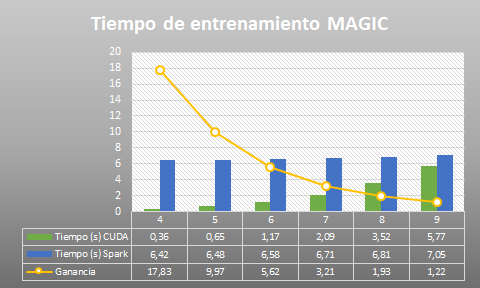
\includegraphics[scale=1.0]{imagenes/magic_times.png}
\caption{Tiempo de entrenamiento y ganacia según profundidad en MAGIC.}
\label{img:magictimes}
\end{figure}

En la figura \ref{img:magictimes} realizamos el mismo análisis para el conjunto de datos \textit{MAGIC Gamma Telescope}. En este caso nos encontramos, en cierta manera, con la situación contraria a la que observábamos en Spambase, el número de muestras considerablemente más elevado (19020) y el número de atributos mucho más reducido (10 más la etiqueta de salida) ponen de manifiesto la velocidad de la ejecución del algoritmo cuando se dan las condiciones ideales para su uso. Cabe destacar que para profundidades muy reducidas, como ocurre en el nivel de profundidad 4, obtenemos una gran ganancia, siendo 17 veces más rápida nuestra implementación que la de \textit{Spark} y manteniendo ganancias considerables para profundidades 6 y 7 (5,62 y 3,21, respectivamente). \\

Puesto que, como comentábamos previamente, ambas implementaciones no hacen exactamente lo mismo es importante observar también las diferencias existentes en términos de precisión para ambos modelos.\\

\begin{figure}[ht]
\centering
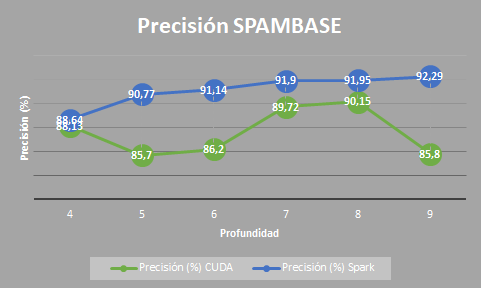
\includegraphics[scale=1.0]{imagenes/spambase_prec.png}
\caption{Precisión según profundidad en SPAMBASE.}
\label{img:spambaseprec}
\end{figure}

La precisión de nuestra implementación según la profundidad (figura \ref{img:spambaseprec}) es considerablemente inferior en la mayoría de niveles de profundidad para el entrenamiento de \textit{Spambase}. La posibilidad de que muestras ruidosas afecten a la calidad de los resultados obtenidos en nuestro modelo es mucho mayor que en el de \textit{Spark} pues no hemos utilizado ninguna técnica de poda más avanzada que limitar la profundidad del árbol generado. Dependiendo del nivel de profundidad, nuestra implementación llega a un rango competitivo de precisión con \textit{Spark} o queda considerablemente por detrás, siendo el caso más claro la profundidad 9 donde \textit{Spark} obtiene una ventaja en precisión del 6,49 \%.\\

\begin{figure}[ht]
\centering
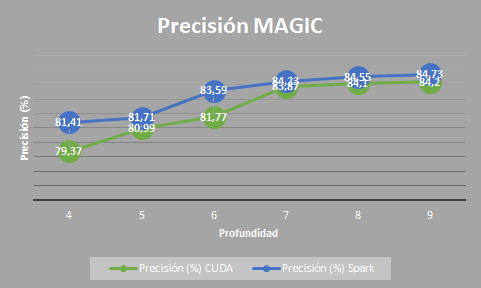
\includegraphics[scale=1.0]{imagenes/magic_prec.png}
\caption{Precisión según profundidad en MAGIC.}
\label{img:magicprec}
\end{figure}

Por otro lado, en la figura \ref{img:magicprec}, podemos observar que no sólo podemos tener problemas por la falta de técnicas de poda avanzadas sino que puesto que ambos algoritmos generan un árbol de decisión de maneras considerablemente distintas habrá situaciones en las que las diferencias entre uno y otro sean mayores y otras en las que sean ambas muy competentes, como en este caso que según el nivel de profundidad la diferencia de precisión varía entre el 0,36 \% y el 2,04 \%.\\

Una vez vistos los puntos fuertes y débiles de nuestra implementación a la hora de probar con nuestro conjunto de \textit{Big Data}, \textit{SUSY}, decidimos en vez de generar un único árbol generar un \textit{random forest} con nuestros árboles de profundidad limitada. En concreto, para el entrenamiento tenemos 4 millones y medio de muestras de 18 atributos más la etiqueta de clasificación. Para nuestro experimento sobre este conjunto hemos generado un \textit{random forest} de 225 árboles utilizando cada uno de ellos 20000 de la muestras presentes en el conjunto y utilizando todos los atributos para entrenar cada árbol. Hemos realizado la misma validación cruzada y realizado el experimento para el sexto y el séptimo nivel de profundidad.

\newpage
\subsection{Tabla de resultados del random forest.}

\begin{table}[ht]
\begin{tabular}{@{}l|cc|cc|@{}}
                             & \multicolumn{2}{c|}{\textit{\textbf{CUDA}}}                                                              & \multicolumn{2}{c|}{\textit{\textbf{SPARK}}}                                                             \\ \midrule
\textit{\textbf{Repetición}} & \multicolumn{1}{l}{\textit{\textbf{Tiempo (s)}}} & \multicolumn{1}{l|}{\textit{\textbf{Precisión (\%)}}} & \multicolumn{1}{l}{\textit{\textbf{Tiempo (s)}}} & \multicolumn{1}{l|}{\textit{\textbf{Precisión (\%)}}} \\ \midrule
\textit{\textbf{1}}          & \textbf{560,48}                                  & 78,12                                                 & 1201,04                                          & \textbf{85,3}                                         \\
\textit{\textbf{2}}          & \textbf{536,01}                                  & 78,14                                                 & 1273,04                                          & \textbf{85,3}                                         \\
\textit{\textbf{3}}          & \textbf{519,96}                                  & 78,24                                                 & 1236,47                                          & \textbf{85,38}                                        \\
\textit{\textbf{4}}          & \textbf{519,47}                                  & 78,15                                                 & 1238,79                                          & \textbf{85,33}                                        \\
\textit{\textbf{5}}          & \textbf{530,59}                                  & 78,13                                                 & 1334,8                                           & \textbf{85,33}                                        \\
\textit{\textbf{6}}          & \textbf{543,35}                                  & 78,11                                                 & 1324,34                                          & \textbf{85,24}                                        \\
\textit{\textbf{7}}          & \textbf{545,54}                                  & 78,15                                                 & 1187,43                                          & \textbf{85,27}                                        \\
\textit{\textbf{8}}          & \textbf{530,74}                                  & 78,1                                                  & 1247,09                                          & \textbf{85,29}                                        \\
\textit{\textbf{9}}          & \textbf{558,46}                                  & 78,18                                                 & 1251                                             & \textbf{85,34}                                        \\
\textit{\textbf{10}}         & \textbf{521,29}                                  & 78,1                                                  & 1268,34                                          & \textbf{85,28}                                        \\ \midrule
\textit{\textbf{MEDIA}}      & {\ul \textit{\textbf{536,59}}}                   & \textit{\textbf{78,14}}                               & \textit{\textbf{1256,23}}                        & {\ul \textit{\textbf{85,31}}}                         \\ \bottomrule
\end{tabular}
\caption{Resultados de validación cruzada en SUSY para profundidad 6.}
\label{tab:susyprof6}
\end{table}

\begin{table}[ht]
\begin{tabular}{@{}l|cc|cc|@{}}
                             & \multicolumn{2}{c|}{\textit{\textbf{CUDA}}}                                                              & \multicolumn{2}{c|}{\textit{\textbf{SPARK}}}                                                             \\ \midrule
\textit{\textbf{Repetición}} & \multicolumn{1}{l}{\textit{\textbf{Tiempo (s)}}} & \multicolumn{1}{l|}{\textit{\textbf{Precisión (\%)}}} & \multicolumn{1}{l}{\textit{\textbf{Tiempo (s)}}} & \multicolumn{1}{l|}{\textit{\textbf{Precisión (\%)}}} \\ \midrule
\textit{\textbf{1}}          & \textbf{583,13}                                  & 78,84                                                 & 1563,44                                          & \textbf{85,78}                                        \\
\textit{\textbf{2}}          & \textbf{559,27}                                  & 78,83                                                 & 1692,27                                          & \textbf{85,8}                                         \\
\textit{\textbf{3}}          & \textbf{584,07}                                  & 78,97                                                 & 1768,84                                          & \textbf{85,88}                                        \\
\textit{\textbf{4}}          & \textbf{548,74}                                  & 78,86                                                 & 1752,11                                          & \textbf{85,82}                                        \\
\textit{\textbf{5}}          & \textbf{561,02}                                  & 78,78                                                 & 1681,44                                          & \textbf{85,82}                                        \\
\textit{\textbf{6}}          & \textbf{574,28}                                  & 78,76                                                 & 1734,05                                          & \textbf{85,72}                                        \\
\textit{\textbf{7}}          & \textbf{572,08}                                  & 78,84                                                 & 1790,56                                          & \textbf{85,77}                                        \\
\textit{\textbf{8}}          & \textbf{580,59}                                  & 78,81                                                 & 1769,53                                          & \textbf{85,76}                                        \\
\textit{\textbf{9}}          & \textbf{576,32}                                  & 78,81                                                 & 1816,56                                          & \textbf{85,82}                                        \\
\textit{\textbf{10}}         & \textbf{592,13}                                  & 78,77                                                 & 1175,02                                          & \textbf{85,76}                                        \\ \midrule
\textit{\textbf{MEDIA}}      & {\ul \textit{\textbf{573,16}}}                   & \textit{\textbf{78,83}}                               & \textit{\textbf{1674,38}}                        & {\ul \textit{\textbf{85,79}}}                         \\ \bottomrule
\end{tabular}
\caption{Resultados de validación cruzada en SUSY para profundidad 7.}
\label{tab:susyprof7}
\end{table}

\newpage
\subsection{Análisis de los resultados del random forest.}
A la hora de realizar este experimento podemos observar cómo los tiempos de ejecución de cada iteración se han disparado para afrontar el problema de mayores dimensiones. La generación de múltiples árboles pequeños nos ha llevado a tardar un promedio de 536,59 segundos para profundidad 6 y 573,16 segundos, es decir un periodo de entre 9 y 10 minutos utilizando la GPU. En el caso de la versión de \textit{Spark} para CPU, en profundidad 6 hemos tardado 1256,23 segundos (unos 20 minutos) y 1674,38 segundos para profundiad 7 (casi 28 minutos), dando lugar a una ganancia promedio de 2,34 para profundidad 6 y de 2,92 para profundidad 7. Mientras que en términos de velocidad de entrenamiento nuestro algoritmo ha sido considerablemente superior incluso incrementando la ganancia al pasar de un nivel de profundidad a otro, hemos de tener en cuenta también la diferencia existente en términos de precisión, que deja nuestra implementación un 7,16 \% de precisión peor para profundidad 6 y un 6,97 \% peor para profundidad 7.\\

\begin{figure}[ht]
\centering
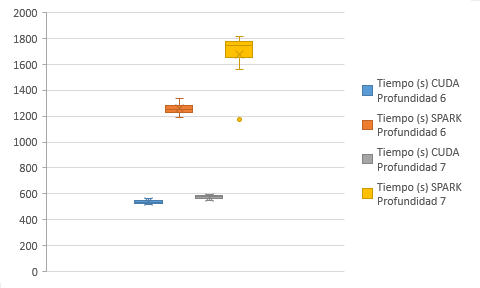
\includegraphics[scale=1.0]{imagenes/boxplot_rf.png}
\caption{Diagrama de cajas y bigotes para el tiempo de entrenamiento del random forest para SUSY.}
\label{img:boxplot}
\end{figure}

De todos los experimentos realizados podemos concluir que mientras que, efectivamente nuestro modelo es más rápido siempre y cuando no generemos árboles demasiado profundos o tengamos una cantidad de atributos muy elevada. En este trabajo, nos hemos centrado en conseguir esa ganancia durante el proceso de entrenamiento. No obstante, pueden ser líneas de trabajo futuras sobre este modelo un análisis específico de los parámetros de profundidad y número de árboles óptimos, la utilización de otros criterios además del utilizado, o el uso del tiempo extra obtenido para mejorar los resultados ya sea con algún preprocesamiento de datos o el uso de criterios de poda más avanzados, entre otros.